An open book in itself is of no use to the proof - a contact structure is needed! 
This section makes the Giroux correspondence explicit by providing a construction that takes an open book as input
and returns a contact structure as output.

Later, it will be important that the resulting contact structure is supported by the open book decomposition.
\begin{definition}\label{def:support}
    Let $(B,p)$ be an oriented open book decomposition of the oriented manifold $M$.
    A contact structure $\xi = \ker \alpha$ on $M$ is said to be \textbf{supported} by the open book decomposition $(B,p)$ of $M$ if
    \begin{enumerate}[(i)]
        \item the contact form $\alpha$ induces the positive orientation of $M$ ($\alpha \wedge (\d \alpha)^n > 0$).
        \item the 2-form $\d \alpha$ induces a symplectic form on each page, defining its positive orientation
        \item the 1-form $\alpha$ induces a positive contact form on $B$, i.e. 
        \[ 
            \alpha|_{TB} \wedge (\d \alpha|_{TB})^{(n-2)} > 0.
        \]
    \end{enumerate}
\end{definition}



\subsection*{Abstract open books}
Instead of defining an open book via a map that induces binding and pages, one can also define it by starting from the page and defining
a "monodromy" map, i.e. a map that determines how the page changes if one follows the page $360^\circ$ around the binding.
This is based on the concept of a mapping torus.

\begin{definition}[mapping torus]
    Let $\Sigma$ be a smooth manifold with boundary $\partial \Sigma$
    and $\phi: \Sigma \to \Sigma$ a diffeomorphism that is equal to the identity close to $\partial \Sigma$.
    The mapping torus $\Sigma(\phi)$ is given by
     $[0,2\pi] \times \Sigma/\sim$ where
     \[
        (2\pi, x) \sim (0, \phi(x)). 
     \]
     The generalized mapping torus requires as additional data a smooth function $\overline{\varphi}: \Sigma \to \mathbb R^+$ that is constant near $\partial \Sigma$. Then,
     \[
        \Sigma_{\overline{\varphi}}(\phi) \coloneqq \mathbb R \times \Sigma/\sim \quad \text{where} \quad  (\theta, x) \sim (\theta - \overline{\varphi}(x), \phi(x)).
     \]
\end{definition}

Starting with a mapping torus $\Sigma(\phi)$, one can construct an abstract open book $M(\phi)$ with binding $\partial \Sigma$ (see \cref{fig:abstract_open_book})
\begin{figure}[ht]
    \includegraphics*[width=\textwidth]{images/abstract_open_book.pdf}
    \caption[abstract open book]{abstract open book}
    \label{fig:abstract_open_book}
\end{figure}

Define
\[
    M(\phi) \coloneqq \left(\Sigma(\phi) \cup \partial D^2 \times \Sigma\right)/\sim
\]
and identify
\[
    [x \in \partial \Sigma, \theta] \sim (r=1, \varphi = \theta, x).
\]


\subsection*{The construction}

Let $\Sigma^{2n}$ be a Liouville domain. 
In particular, it is a compact manifold admitting an exact symplectic form $\omega = \d \beta$ 
s.t. on the boundary $\partial \Sigma$, a contact form $\beta_\partial$ is induced.
Let the boundary be connected (i.e. the binding is also connected).
Let the monodromy map $\phi$ be an exact symplectomorphism of $(\Sigma, \omega)$,
equal to the identity near the boundary $\partial \Sigma$ (exactness is not necessary according to \cite{Geiges08}, as it can be obtained via a suitable isotopy of the symplectomorphism).
An exact symplectomorphism $\phi$ of $(\Sigma, \omega)$ is such that
\[
    \phi^*(\beta) - \beta \eqqcolon \d \overline{\varphi}  
\]
is exact, i.e. there exists such a function $\overline{\varphi}$ on $\Sigma$ (of course only defined up to adding a locally constant function. Choose it in such a way that it only takes positive values).
The 1-form 
\[
    \alpha \coloneqq \beta + \d \varphi
\]
is a contact form on $\mathbb R \times \Sigma$:
\[
    \alpha \wedge (\d \alpha)^{n} = (\beta + \d \varphi)\wedge \underbrace{(\d \beta)^n}_{\eqqcolon \Omega} = \beta \wedge \Omega + \d \varphi \wedge \Omega = \d \varphi \wedge \Omega,
\]
where $\Omega$ is a volume form on $\Sigma$ (as $\beta$ is a symplectic form).
The term $\beta \wedge \Omega$ vanishes because both are forms on $\Sigma$, but $\Omega$ is already a top-level form.
The resulting form is a wedge product of two volume forms on the product manifolds and therefore a volume form on $\mathbb R \times \Sigma$.

Now consider the transformation that induces the generalized mapping torus
\[
    F \coloneqq (\varphi, x) \mapsto (\varphi - \overline{\varphi}(x), \phi(x)).    
\]
Remember that $\varphi$ only takes positive values, i.e. the mapping torus is welldefined.
The 1-form $\alpha$ is invariant under this transformation:
\begin{align*}
    F^*(\alpha) &= F^*(\beta) + F^*(\d \varphi)&&|\;\beta\text{ is independent of }\varphi\\
    &= \phi^*(\beta) + \d F(\varphi)&&|\text{ definition of }\overline{\varphi}, F\\
    &= \beta + \d\overline{\varphi} + \d \varphi - \d \overline{\varphi}\\
    &= \alpha.
\end{align*}
It follows that $\alpha$ descends to a contact form on $\Sigma_{\overline{\varphi}}(\phi)$. 

In the following, it will be necessary to have an adapted gluing construction for the abstract open book coming from a generalized mapping torus.
The page $\Sigma$ is Liouville, i.e. there exists a Liouville vector field $X$ which is transversal to the boundary $\partial \Sigma$.
This vector field induces a coordinate $s$ on a collar neighborhood of the boundary $[-1,0] \times \partial \Sigma$.
Then, the symplectic form is given by $\d \left(e^s\beta_\partial\right)$ where $s$ is the collar parameter, i.e. $X = \partial s$.

Close to $\partial \Sigma$, $\phi$ is equal to the identity and therefore $\d \overline{\varphi}$ is locally constant (hence constant, as $\partial \Sigma$ is connected).
Parametrize the neighborhood so that $\overline{\varphi}$ is constant on $[-1,0]\times \partial \Sigma$.

Now, take a look at
\[
    M \coloneqq \left(\Sigma_{\overline{\varphi}}(\phi)\; \dot\cup\; \left(\partial D_2^2 \times \Sigma\right)\right)/\sim.
\]
\begin{figure}
    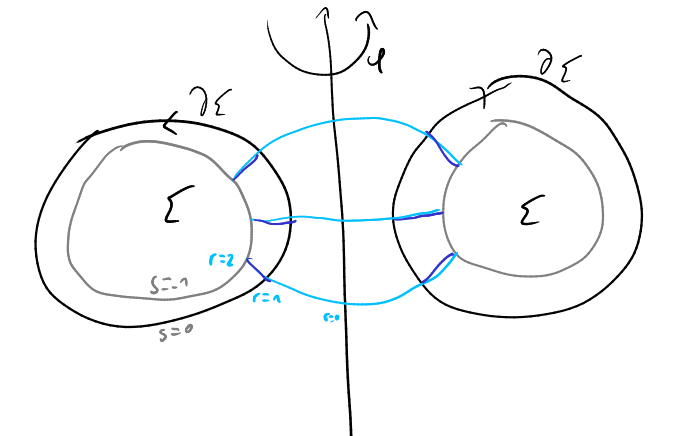
\includegraphics[width=\textwidth]{images/abstract_open_book_gluing.png}
    \caption[Gluing an abstract open book]{Detailled gluing process of the generalized abstract open book}
    \label{fig:abstract_open_book_gluing}
\end{figure}

A simple linear reparametrization will make the notation a lot easier: As $\overline{\varphi}$ is constant on the neighborhood under consideration, just pretend that $\overline{\varphi} = 2\pi$.
Furthermore, parametrize the boundary $\partial \Sigma$ with $\theta \in S^1$.
Then identify 
\[
    (s, \theta, \varphi) \in [-1,0] \times \partial \Sigma \times S^1 \subset \Sigma_{\overline{\varphi}}(\phi)
\]
with
\[
    (\theta, s = 1-r, \varphi) \in \partial \Sigma \times D_2^2 \eqqcolon \mathcal{N}
\]
where $(r, \varphi)$ are polar coordinates on $D_2^2$, i.e. a collar neighborhood of $\Sigma$ is identified with an annulus in $D_2^2$.
(See \cref{fig:abstract_open_book_gluing})

Now choose the ansatz
\[
    \alpha_\text{ext} \coloneqq h_1(r) \beta_\partial + h_2(r) \d\varphi.
\]
for the extension of the contact form over $\mathcal{N}$.
On the gluing area (i.e. $1 \le r \le 2$), $\alpha_\text{ext}$ has to agree with $\alpha = \beta + \d \varphi = e^s \beta_\partial + \d \varphi$,
i.e.
\[
    h_1(r) = e^s = e^{1-r} \qquad h_2(r) = 1.
\]
In order to ensure smoothness at $r=0$, set $h_1(r) = 2 - r^2$ and $h_2(r) = r^2$ in a small neighborhood of $r = 0$. Then,
\[
    \alpha_\text{ext}|_0 = 2\beta_\partial
\]
Further,
\[
    \d \alpha_\text{ext} = h_1'(r)\d r\wedge \beta_\partial + h_1(r) \d \beta_\partial + h_2'(r) \d r \wedge \d\varphi.
\]
and
\[
    (\d \alpha_\text{ext})^n = n\cdot \d r\wedge (h_1'(r) \beta_\partial + h_2'(r) \d\varphi) \cdot h_1(r)^{n-1}(\d \beta_\partial)^{n-1} + \underbrace{h_1(r)^n (\d \beta_\partial)^n}_{=0},
\]
where the second term vanishes because $(\d \beta_\partial)^n$ is a $2n$-form on $\partial \Sigma^{2n-1}$.
% the first and third term together can occur at most once in a term becuase of the dr
% as dbeta is a two-form, the order doesn't matter and it commutes with the other terms
Finally,
\begin{align*}
    \alpha_\text{ext} \wedge (\d \alpha_\text{ext})^n =& \;h_1(r)n h_1(r)^{n-1} h_2'(r) \cdot&&\beta_\partial \wedge \d r \wedge \d \varphi \wedge (\d\beta_\partial)^{n-1}\\
    &+ h_2(r)n h_1(r)^{n-1}h_1'(r) \cdot&&\d \varphi \wedge \d r \wedge \beta_\partial \wedge (\d\beta_\partial)^{n-1}\\
    =& n h_1(r)^{n-1}(h_1h_2'(r) - h_2h_1'(r)) \cdot &&\beta_\partial \wedge (\d\beta_\partial)^{n-1} \wedge \d r \wedge \d \varphi\\
    =& n h_1(r)^{n-1}\det \begin{pmatrix}
        h_1(r) & h_2(r)/r\\
        h_1'(r) & h_2'(r)/r
    \end{pmatrix} \cdot &&\beta_\partial \wedge (\d\beta_\partial)^{n-1} \wedge r \d r \wedge \d \varphi\\
\end{align*}
As $\beta_\partial$ is a contact form on $\partial \Sigma$, $\beta_\partial \wedge (\d\beta_\partial)^{n-1}$ is a positive volume form on $\partial \Sigma$. 
Furthermore, $r \d r\wedge \d \varphi$ is a positive volume form on the disk $D_2^2$. 
As a result, the right term of the result is a volume form on $\mathcal{N} = \partial \Sigma \times D_2^2$.
The left term shows that $h_1(r)$ musn't have any zeros for $r \in [0,2]$ and that $(h_1(r), h_2(r))$ must never be parallel to $(h_1'(r), h_2'(r))$, i.e.
\[
    h_1(r)^{n-1}\det \begin{pmatrix}
        h_1(r) & h_2(r)/r\\
        h_1'(r) & h_2'(r)/r
    \end{pmatrix} > 0 \qquad \forall r \in [0,2].
\]
(Close to zero, the determinant is given by $2 \cdot 2 - 0 \cdot 0 = 4 > 0$).
Figure 4.7 in \cite{Geiges08} proves the existence of such a pair of functions $h_1$ and $h_2$.


In total, $\alpha_\text{ext}$ induces the correct orientation on the extension and,
as $M$ is connected and orientable, on all of $M$.
In particular, condition (i) of \cref{def:support} holds and $\alpha \wedge (\d \alpha)^n = \d \varphi \wedge \Omega$ is a positive volume form on the mapping torus. 

Recall that $\omega$ is the symplectic form on $\Sigma$.
As $\Omega = (\d \beta)^n = \omega^n$, it is a $2n$-form and hence $\Omega$ is a positive volume form on $\Sigma$. 
Thus, on $\Sigma$, $\d \alpha = \d \beta = \omega$ is a symplectic form that induces the positive orientation of $\Sigma$. 
On $\mathcal{N}$, it is necessary to check that the form induced by $\d \alpha_\text{ext}$ on the pages is symplectic with the right orientation.
Inside $\mathcal{N}$, a page is given by the condition $\varphi = \mathrm{const}$, i.e. $\d \varphi = 0$.
Also,
\begin{align*}
    (\d \alpha_\text{ext})^n &= n\cdot \d r\wedge (h_1'(r) \beta_\partial + h_2'(r) \d\varphi) \cdot h_1(r)^{n-1}(\d \beta_\partial)^{n-1}\\
    &= n h_1'(r)h_1(r)^{n-1} \d r \wedge \beta_\partial \wedge (\d \beta_\partial)^{n-1}
\end{align*}

A positive volume form on $\Sigma$ must be positive on $- \partial_r, \mathfrak{b}$ where $\mathfrak{b}$ is a positive basis of a point in $\partial \Sigma$.
As $\beta_\partial \wedge (\d \beta_\partial)^{n-1}$ is a positive volume form on $\partial \Sigma$, it follows
\begin{align*}
    (\d \alpha_\text{ext})^n(- \partial_r, \mathfrak{b}) &= \underbrace{n h_1(r)^{n-1}}_{\eqqcolon A > 0} \cdot h_1'(r) \d r(-\partial_r) \wedge \underbrace{\left[\beta_\partial \wedge (\d \beta_\partial)^{n-1}\right](\mathfrak{b})}_{\eqqcolon B > 0}\\
    &= AB \cdot h_1'(r) \cdot -1\\
    &> 0,
\end{align*}
where in the last line $h_1'(r) = \frac{\d}{\d r}(2 - r^2) = -2r < 0$.
This verifies condition (ii) inside $\mathcal{N}$ and outside $\mathcal{N}$, on $\Sigma$. As a result, is must hold on the whole page.
Condition (iii) follows from the fact that on $B$, $\alpha_\text{ext} = 2 \beta_\partial$ which is a positive contact form on $\partial \Sigma$ and therefore also on $B$.

This concludes the construction of a contact structure supported by a starting open book.
As this construction will be applied to the Milnor open book, one musg check that it satisfies all requirements for the construction.
Every open book is an abstract open book. For the Milnor open book, the pages are Weinstein and in particular Liouville.
The binding is connected for $\dim B \geq 3$, i.e. as soon as the open book composition has $\dim \geq 5$.
As this thesis only considers the case with $\dim S^{2n+1} \geq 7$ and the Bourgeois construction will add 2 dimensions, this suffices
in all cases that are considered here. 
The conditions on the monodromy are also satisfied as the abstract open book comes from an open book. \underline{Really?}